\documentclass{beamer}
\usepackage{amsmath, amsfonts, mathtools, amsthm, amssymb}
\usepackage[bb=boondox]{mathalfa}

\usepackage{xcolor}
\usepackage{changepage}


\usefonttheme[onlymath]{serif}



\definecolor{darkgreen}{HTML}{3C6A12}
\definecolor{lightgreen}{HTML}{F0F7E0}

\setbeamercolor{frametitle}{fg=lightgreen, bg=darkgreen}

\setbeamertemplate{itemize item}{\color{darkgreen}$\blacksquare$}
\setbeamertemplate{itemize subitem}{\color{darkgreen}$\blacktriangleright$}
\author{Ole W. Kaa (olkaa21@student.sdu.dk)}



\newcommand\Wider[2][3em]{%
\makebox[\linewidth][c]{%
  \begin{minipage}{\dimexpr\textwidth+#1\relax}
  \raggedright#2
  \end{minipage}%
  }%
}

\beamertemplatenavigationsymbolsempty

\begin{document}


\begin{frame}{}
    \title{\huge \color{darkgreen} Numerical integration of\par highly oscillatory functions}
    \titlepage
\end{frame}

\begin{frame}{Motivation}
    \begin{itemize}
        \setlength\itemsep{1em}
        \item Oscillatory Functions
        \item Numerically integrate
        \item Sign problem
    \end{itemize}
\end{frame}


\begin{frame}{One-Dimensional Function}
    \noindent\begin{minipage}{0.40\textwidth}
        \(f(x)=e^{-x^2} \cos(\lambda x)\)\\
        
        \vspace{1em}
        
        \(\int_{-\infty}^\infty f(x)\,dx = \sqrt{\pi}e^{-\frac{\lambda^2}{4}} \)\\

    \end{minipage}%
    \hfill%
    \begin{minipage}{0.60\textwidth}\raggedleft
        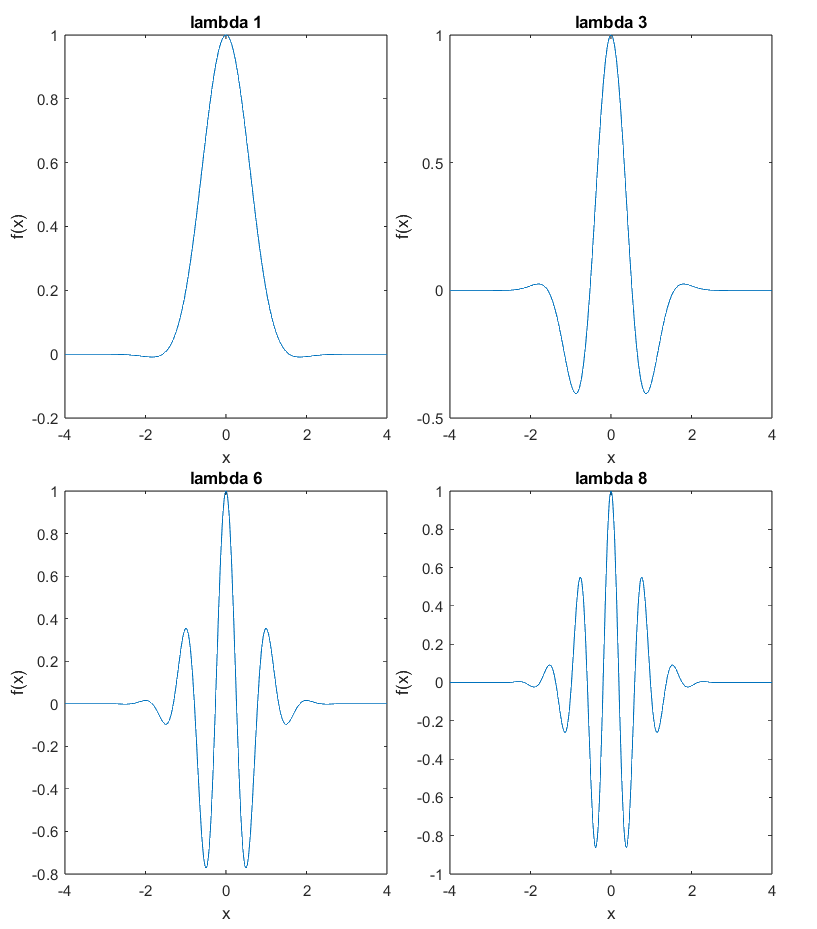
\includegraphics[width=\linewidth]{Graphs/1Dfunc.png}
    \end{minipage}
\end{frame}

\begin{frame}{Multi/Two-Dimensional Function}
    \noindent\begin{minipage}{0.40\textwidth}
        \(f(\mathbf{x})=\)
        
        \qquad\(e^{-\sum_{i=1}^n x_i^2}\)
        
        \qquad\(\cdot\cos\Big(\sum_{i=1}^n \lambda_i x_i\Big) \)
        
        \vspace{1em}
        
        \(\int_{\mathbb{R}^n}f(\mathbf{x})\, d\mathbf{x}=\)
        
        \qquad\(\pi^{\frac{n}{2}} e^{-\frac{1}{4}\sum_{i=1}^n\lambda_i^2} \)\\

    \end{minipage}%
    \hfill%
    \begin{minipage}{0.60\textwidth}\raggedleft
        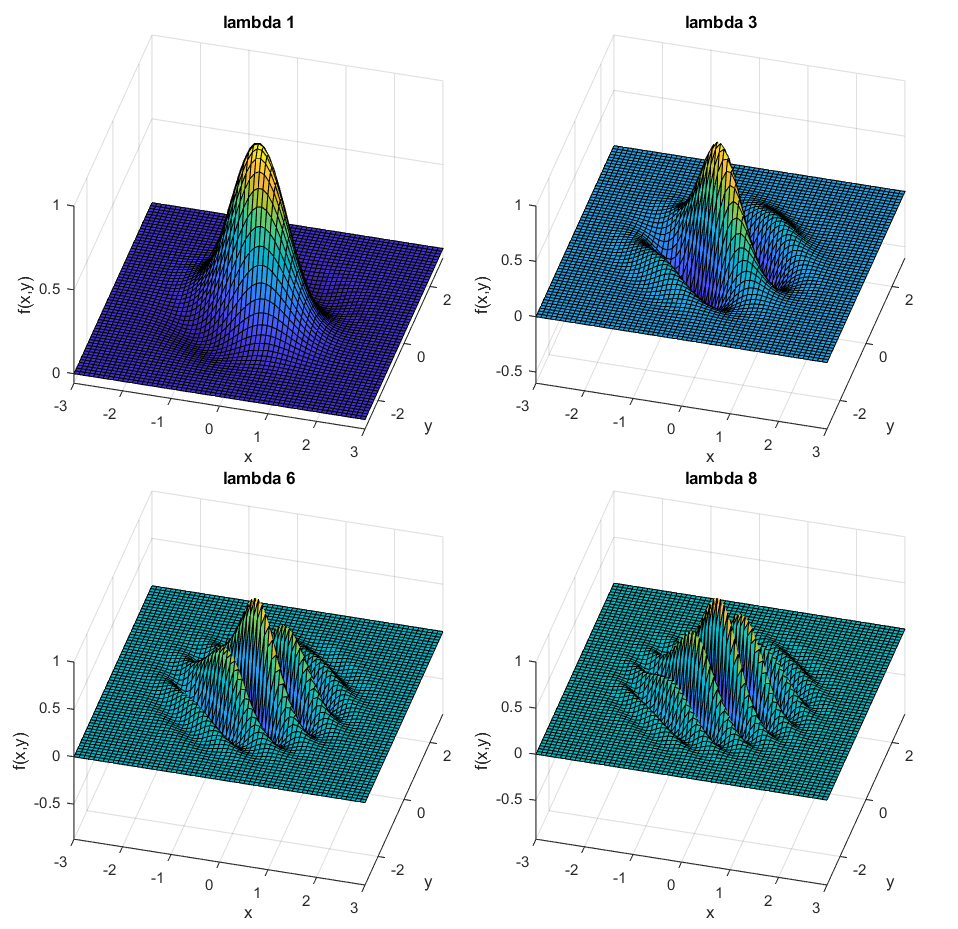
\includegraphics[width=\linewidth]{Graphs/2Dfunc.png}
    \end{minipage}
\end{frame}

\begin{frame}{Numerical Integration}
    \begin{itemize}
        \setlength\itemsep{1em}
        \item Newton-Cotes Methods
        \begin{itemize}
            \item Midpoint rule
            \item Trapezoid rule
            \item Simpson's rule
        \end{itemize}
        \item Monte Carlo Integration Methods
        \begin{itemize}
            \item Simple sampling
            \item Importance sampling
        \end{itemize}
        \item \(N=2^{i},\quad i=4,5,\ldots,29\)
        \item \(\lambda \in\{1,3,6,8\}\)
        \item Even Function 
    \end{itemize}
\end{frame}

\begin{frame}{One Dimension: \(\lambda\in\{1,3\}\)}
    \Wider{\centering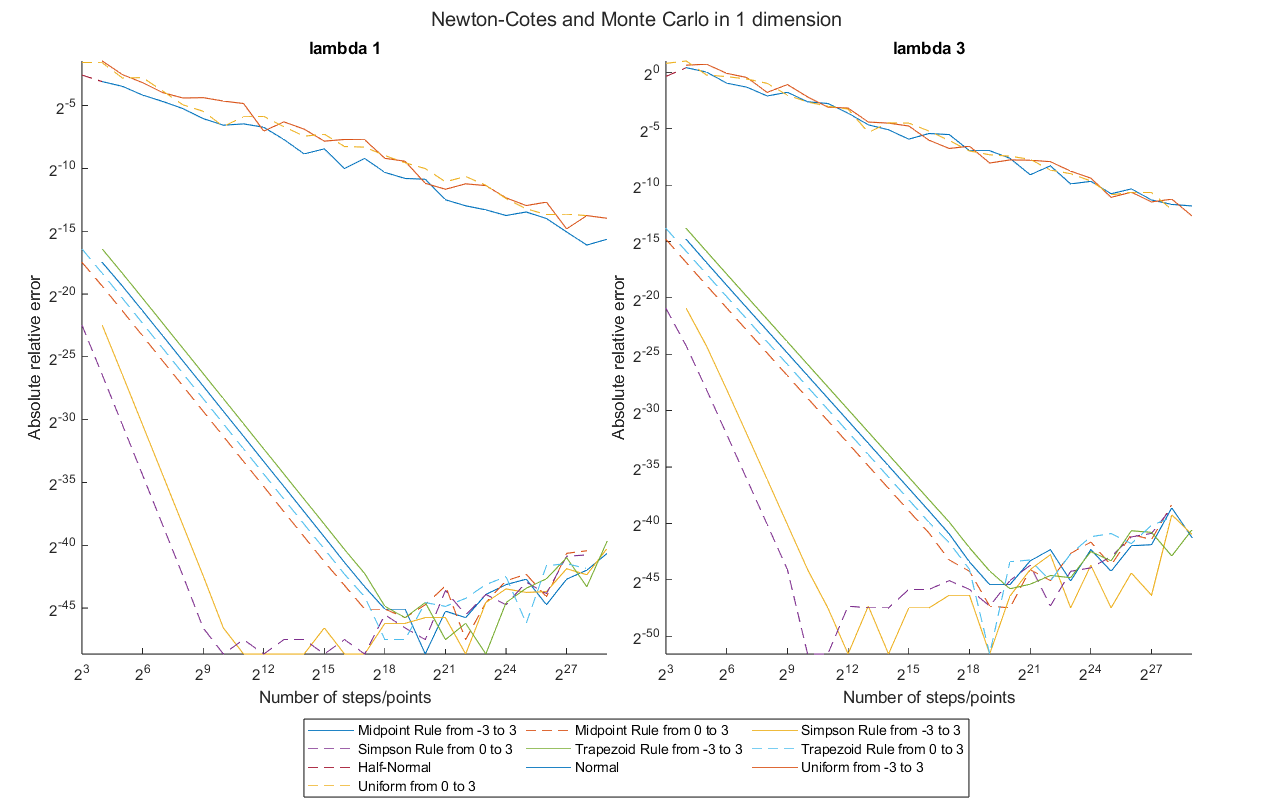
\includegraphics[scale=0.35]{Graphs/NCVMC1d_1_3.png}}
\end{frame}

\begin{frame}{One Dimension: \(\lambda\in\{6,8\}\)}
    \Wider{\centering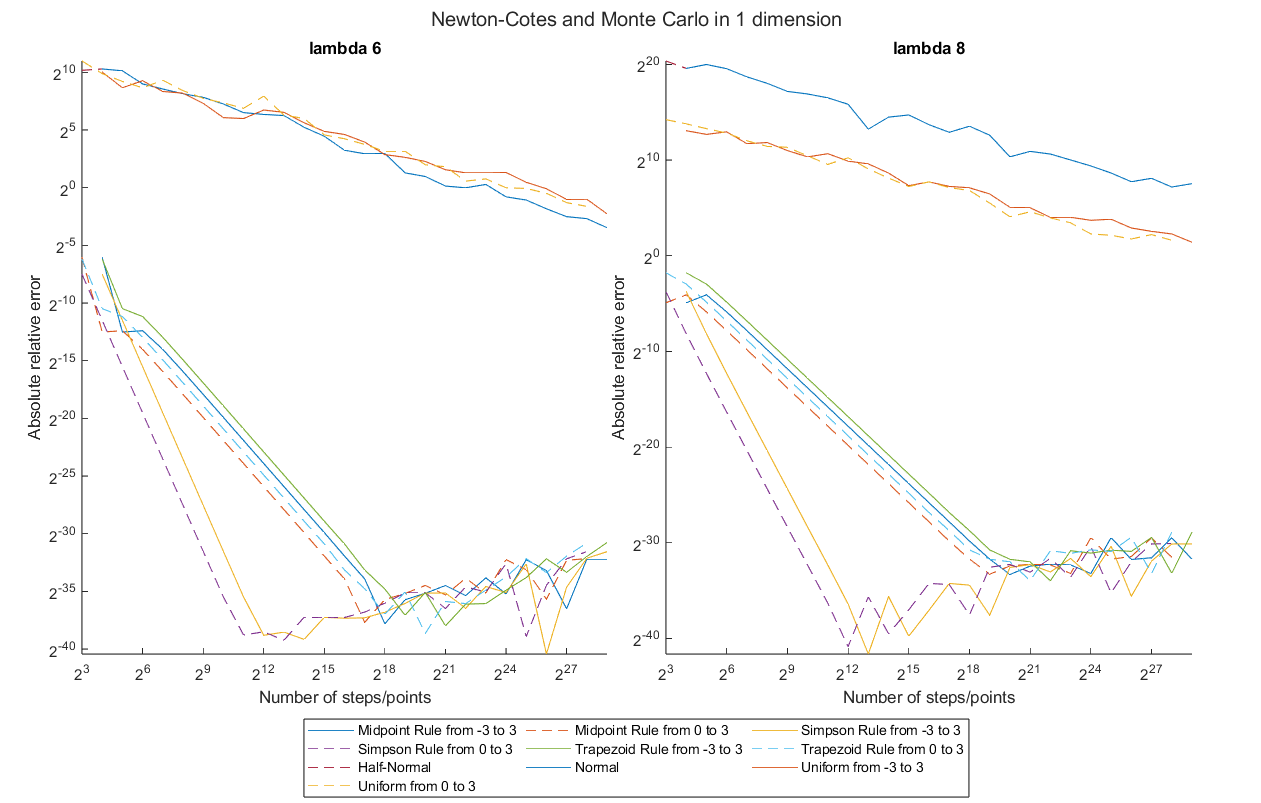
\includegraphics[scale=0.35]{Graphs/NCVMC1d_6_8.png}}
\end{frame}


\begin{frame}{Two Dimensions: \(\lambda\in\{1,3\}\)}
    \Wider{\centering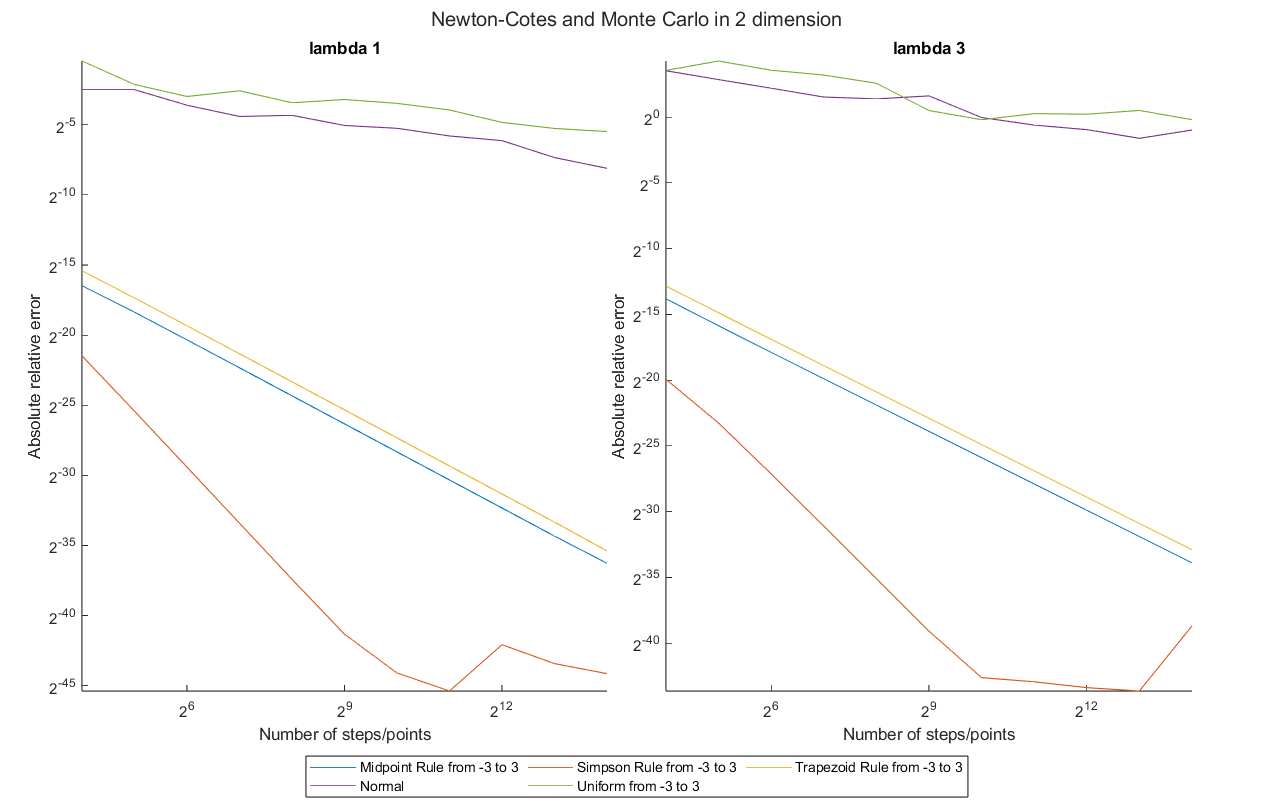
\includegraphics[scale=0.35]{Graphs/NCVMC2d_1_3.png}}
\end{frame}

\begin{frame}{Two Dimensions: \(\lambda\in\{6,8\}\)}
    \Wider{\centering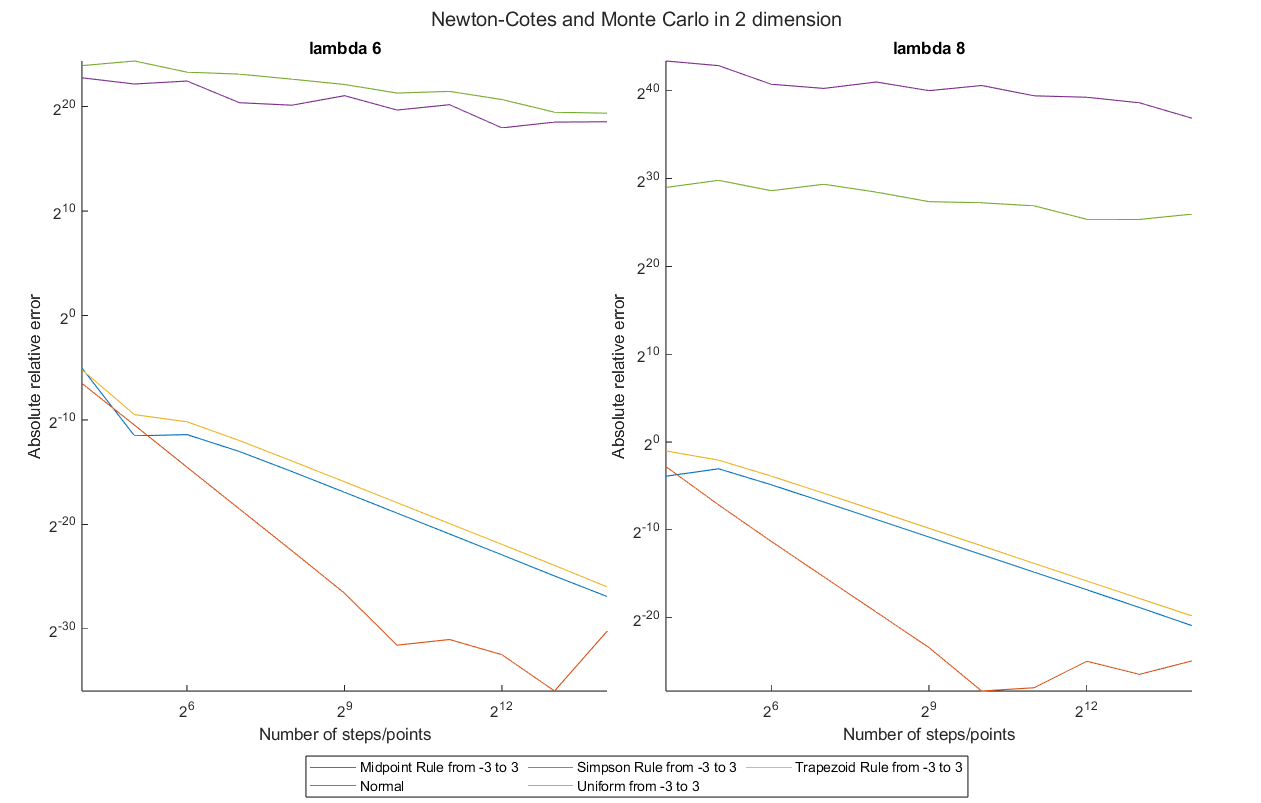
\includegraphics[scale=0.35]{Graphs/NCVMC2d_6_8.png}}
\end{frame}


\begin{frame}{Discussion / Conclusion}
    \begin{itemize}
        \setlength\itemsep{1em}
        \item Value of \(\lambda\)
        \item Newton-Cotes Methods
        \item Monte Carlo Integration Methods
        \item Newton-Cotes Vs. Monte Carlo
        \item Computational Complexity Vs. Error
        \item Machine Precision
    \end{itemize}
\end{frame}

\end{document}